\documentclass[11pt,a4paper]{article}

\usepackage[T1]{fontenc}
\usepackage[utf8]{inputenc}
\usepackage{lmodern}
\usepackage[margin=0.85in]{geometry}
\usepackage{amsmath,amssymb}
\usepackage{booktabs}
\usepackage{graphicx}
\usepackage{hyperref}
\usepackage{algorithm}
\usepackage{algpseudocode}
\usepackage{microtype}
\usepackage{xcolor}
\usepackage{caption}
\usepackage{float}
\usepackage{placeins}
\usepackage{needspace}
\hypersetup{colorlinks=true,linkcolor=black,citecolor=black,urlcolor=blue}
\setlength{\textfloatsep}{6pt plus 1pt minus 2pt}
\setlength{\floatsep}{6pt plus 1pt minus 2pt}
\setlength{\intextsep}{6pt plus 1pt minus 2pt}
\captionsetup{font=small,skip=3pt}
\setlength{\abovedisplayskip}{6pt plus 2pt minus 2pt}
\setlength{\belowdisplayskip}{6pt plus 2pt minus 2pt}
\setlength{\abovedisplayshortskip}{4pt plus 1pt minus 1pt}
\setlength{\belowdisplayshortskip}{4pt plus 1pt minus 1pt}
\algnewcommand{\Input}{\item[\textbf{Input:}]}
\algnewcommand{\Output}{\item[\textbf{Output:}]}

\title{Reinforcement Learning for Test-Time Compute Allocation\\
in Latent Program Networks\\[0.35em]
\large A Controlled Stop-or-Continue Prototype on Frozen Pattern Models}
\author{Cl\'ement Callaert\\
CentraleSup\'elec, Universit\'e Paris-Saclay\\[0.25em]
\textit{Research report prepared for discussion with Nathana\"el Fijalkow}}
\date{}

\begin{document}
\maketitle

\begin{abstract}
Latent Program Networks (LPNs) allocate test-time compute by optimizing a
latent program against a support-set likelihood before decoding a query
prediction~\cite{macfarlane2024lpn}.
A fixed search budget can waste steps on instances already solved by the
encoder initialization.
We formulate adaptive allocation as a finite-horizon stop-or-continue Markov
decision process: the policy observes only search diagnostics and never the
query target, then either stops and decodes or applies one clipped SGD latent
update.
A linear Bernoulli policy is trained with REINFORCE on offline deterministic
search trajectories from frozen \texttt{pattern\_2d} checkpoints~0 and~1, and
evaluated on held-out checkpoint~2.
On 96 leave-one-out episodes from 24 procedural tasks, Fixed-5 and RL with
$\lambda{=}0$ both obtain exact match $0.90625$, while RL uses $4.281$ mean
steps instead of $5.000$.
Gradient-norm stopping is stronger at the same exact match with $3.438$ mean
steps.
This is \texttt{pattern\_2d} sandbox evidence, not an ARC result.
\end{abstract}

% =====================================================================
\section{Motivation}
% =====================================================================

The research question is:
\emph{Can a learned controller allocate test-time latent-search computation
more effectively than a fixed budget or a simple stopping heuristic?}

Nathana\"el Fijalkow proposed reading the LPN paper, reusing its code, and
asking whether reinforcement learning can improve test-time compute.
The object is allocation of inference-time search steps on a frozen model, not
a new encoder/decoder.

Fixed-$K$ search is often inefficient: some tasks are solved at $K{=}0$, others
need several updates, so a constant horizon can overspend on easy episodes and
under-search hard ones.
We pursue two objectives: preserve query exact match and reduce expected search
cost.
Neither is claimed solved here.

% =====================================================================
\section{Latent Program Search}
% =====================================================================

Let a task provide a support set
$\mathcal{D}_{s}=\{(x_i,y_i)\}_{i=1}^{N}$
and a query input $x_{\mathrm{query}}$ with hidden target $y_{\mathrm{query}}$.
A frozen LPN with parameters $\theta$ encodes each support pair through a
variational encoder
$(\mu_i,\log\sigma_i^2)=E_\theta(x_i,y_i)$
and samples
\begin{equation}
z_i
=
\mu_i
+
\exp\!\left(\tfrac12\log\sigma_i^2\right)\varepsilon_i,
\qquad
\varepsilon_i\sim\mathcal{N}(0,I).
\end{equation}
In the default mean-latent case the initial context is
$z_0=\frac1N\sum_{i=1}^{N}z_i$.

Search maximizes a support score.
Writing $r_i$ and $c_i$ for the output row and column counts, and
$\Omega_i$ for the valid output cells of pair $i$,
\begin{equation}
\begin{aligned}
S(z;\mathcal{D}_s)
=
\sum_{i=1}^{N}
\Big[
&\log p_\theta(r_i\mid x_i,z)
+
\log p_\theta(c_i\mid x_i,z)\\
&+
\tfrac{1}{|\Omega_i|}
\sum_{u\in\Omega_i}
\log p_\theta(y_{i,u}\mid x_i,z)
\Big].
\end{aligned}
\end{equation}
Shape terms constrain dimensions; the cell likelihood constrains content;
averaging over $|\Omega_i|$ prevents larger grids from dominating; the sum over
pairs identifies a latent compatible with the observed transformation.

One clipped SGD ascent step uses Optax \texttt{clip\_by\_global\_norm}$(1.0)$
then SGD at learning rate $\eta$, presenting $-\nabla_z S$ so descent implements
ascent. Equivalently,
\begin{equation}
g_t=\nabla_z S(z_t;\mathcal{D}_s),\quad
\widetilde{g}_t=\frac{g_t}{\max(1,\|g_t\|_2)},\quad
z_{t+1}=z_t+\eta\widetilde{g}_t.
\end{equation}
LPN retains all iterates and returns a best-so-far latent
\begin{equation}
z^\star_K
\in
\operatorname*{arg\,max}_{z\in\{z_0,\ldots,z_K\}}
S(z;\mathcal{D}_s).
\end{equation}
The query prediction is
$\widehat{y}=D_\theta(x_{\mathrm{query}},z^\star_K)$
with fixed greedy decoding.
Stopping at step $K$ does not imply returning $z_K$: the system returns the
highest support-scoring iterate observed so far.

Query exact match is
\begin{equation}
\operatorname{EM}(\widehat{y},y)
=
\mathbf{1}
\!\left[
\operatorname{shape}(\widehat{y})=\operatorname{shape}(y)
\land
\widehat{y}=y
\right].
\end{equation}

% =====================================================================
\section{Reinforcement-Learning Formulation}
% =====================================================================

We cast adaptive search as a finite-horizon MDP
$\mathcal{M}=(\mathcal{S},\mathcal{A},P,R,H)$
with horizon $H{=}5$ and action set
$\mathcal{A}=\{\texttt{stop},\texttt{continue}\}$.
Action $a_t{=}0$ stops and decodes with the current best latent.
Action $a_t{=}1$ applies one original clipped SGD step.

The full Markov state contains at least
$s_t=(z_t,z_t^\star,S_t,S_t^\star,g_t,t,H)$.
The policy observes only the eight-dimensional diagnostic vector
\begin{equation}
o_t
=
\Big[
\tfrac{t}{H},\,
\tfrac{H-t}{H},\,
S_t,\,
S_t-S_{t-1},\,
S_t^\star-S_{t-1}^\star,\,
\|g_t\|_2,\,
\|z_t\|_2,\,
\|z_t-z_{t-1}\|_2
\Big].
\end{equation}
Support score, gradient norm, latent norm, and latent-update norm are
normalized with training-split statistics (zero variance replaced by $1$).
Step fractions are already scaled by $H$.
The query target is forbidden: $y_{\mathrm{query}}\notin o_t$.

An episode $\tau$ ends when the policy stops or the horizon is reached.
Let $T(\tau)$ be the number of executed search steps.
The terminal reward is
\begin{equation}
R(\tau)
=
\mathbf{1}\!\left[\widehat{y}_\tau=y_{\mathrm{query}}\right]
-
\lambda\,T(\tau).
\end{equation}
With $\lambda{=}0$ the objective is terminal exact match only; $\lambda{>}0$
penalizes computation and can make immediate stopping optimal.
We do not describe $\lambda{=}0$ as optimizing compute.

The policy is a linear Bernoulli classifier over the stop action,
\begin{equation}
p_\phi(\texttt{stop}\mid o_t)=\sigma(w^\top o_t+b),\qquad
p_\phi(\texttt{continue}\mid o_t)=1-p_\phi(\texttt{stop}\mid o_t),
\end{equation}
with policy parameters $\phi=(w,b)$, distinct from frozen LPN parameters
$\theta$.
Training uses the REINFORCE estimator~\cite{williams1992reinforce}
\begin{equation}
\nabla_\phi J(\phi)
=
\mathbb{E}_{\tau\sim\pi_\phi}
\!\left[
\bigl(R(\tau)-b_{\mathrm{avg}}\bigr)
\sum_{t=0}^{T(\tau)}
\nabla_\phi\log\pi_\phi(a_t\mid o_t)
\right],
\end{equation}
where $b_{\mathrm{avg}}$ is a moving-average return baseline, distinct from the
policy bias $b$.
The baseline preserves the estimator expectation and reduces variance when
correlated with the return; it does not guarantee low variance.
Because the only non-terminal action follows fixed deterministic SGD of the
frozen LPN, trajectories can be precomputed offline and the policy selects a
stopping time.
This is restricted optimal stopping, not a general RL environment with
policy-dependent transitions.

% =====================================================================
\section{Implementation}
% =====================================================================

The stack adds algorithmic compute counters; closed-loop adaptive search;
deterministic fixed-horizon trajectory extraction; a stop/continue environment;
training-split observation normalization; a linear Bernoulli policy; REINFORCE
with Adam, gradient clipping, and an optional entropy bonus; and a matched
evaluation harness.

\begin{algorithm}[H]
\caption{RL-controlled latent search}
\label{alg:rlsearch}
\small
\begin{algorithmic}[1]
\Input support $\mathcal{D}_s$, query $x_{\mathrm{query}}$, frozen LPN $\theta$, horizon $H$, policy $\pi_\phi$
\State Encode support pairs; construct $z_0$; score $S_0$; set $z_0^\star\!\leftarrow\!z_0$
\For{$t=0,\ldots,H$}
  \State Build $o_t$ (no query target); select $a_t\sim\pi_\phi(\cdot\mid o_t)$
  \If{$a_t=\texttt{stop}$}
    \State Decode $\widehat{y}=D_\theta(x_{\mathrm{query}},z_t^\star)$; \textbf{terminate}
  \ElsIf{$t=H$}
    \State Force stop: decode with $z_t^\star$; \textbf{terminate}
  \Else
    \State One clipped SGD step $\to z_{t+1}$; update $z^\star$, scores, counters
  \EndIf
\EndFor
\end{algorithmic}
\end{algorithm}

Trajectory-control parity against upstream fixed-$K$ search for
$K\in\{0,1,5\}$ (matched keys, $\eta{=}0.1$) gave bit-identical decoded grids
and shapes, with selected contexts numerically close (max abs.\ difference about
$10^{-4}$ to $4{\times}10^{-4}$; tests use $\mathrm{atol}{=}\mathrm{rtol}{=}10^{-3}$).
This validates functional parity of finals, not bitwise equality of every
internal upstream gradient (those intermediates are not exported).

% =====================================================================
\section{Experimental Setup}
% =====================================================================

All experiments freeze the base LPN and use in-family procedural
\texttt{pattern\_2d} / \texttt{lpn-2d} tasks.
They do not establish ARC-AGI progress, OOD generalization, or statistical
significance.
The goal is to test whether RL can control latent-search computation.

\begin{table}[H]
\centering
\caption{Experimental configuration. Sources:
\texttt{settingB\_ckpt2\_ds0\_len24\_eval\_20260723.json} and
\texttt{settingB\_penalty0.00\_20260723/train\_summary.json}.}
\label{tab:setup}
\setlength{\tabcolsep}{3.5pt}
\footnotesize
\begin{tabular}{@{}ll@{}}
\toprule
Item & Value \\
\midrule
Base model & Frozen \texttt{pattern\_2d} LPN \\
Frozen checkpoints & Seeds 0, 1, 2 \\
Search optimizer / lr & Clipped SGD (norm 1.0) / $0.1$ \\
Horizon $H$ / obs.\ dim. & $5$ / $8$ \\
Policy / algorithm & Linear Bernoulli / REINFORCE + baseline \\
Reward & $\operatorname{EM}-\lambda T$ \\
Train / val / test seeds & 1000--1001 / 2000 / 0 \\
Train / test checkpoints & 0, 1 / 2 \\
Final tasks / episodes & 24 / 96 leave-one-out \\
Accelerator / JAX / Flax & \texttt{cuda:0} / 0.6.0 / 0.10.2 \\
\bottomrule
\end{tabular}
\end{table}

\begin{table}[H]
\centering
\caption{Procedural splits for Setting~B. Each task has four pairs; leave-one-out
evaluation yields four episodes per task (correlated).}
\label{tab:splits}
\small
\begin{tabular}{@{}llll@{}}
\toprule
Split & Procedural seeds & LPN checkpoints & Length \\
\midrule
Train & 1000, 1001 & 0, 1 & 8 \\
Validation & 2000 & 0, 1 & 8 \\
Final test & 0 & 2 & 24 \\
\bottomrule
\end{tabular}
\end{table}

Penalty selection used validation return; selected $\lambda{=}0$, which does not
explicitly penalize compute (any step cut is a side effect).
Policy training: learning rate $0.01$, batch $32$, $100$ updates, entropy
coefficient $0.01$, policy seed~$0$.
Evaluation stops when $p_\phi(\texttt{stop}\mid o_t)\ge 0.5$.
Over $M{=}96$ episodes,
$\widehat{\operatorname{EM}}=\frac1M\sum_j\operatorname{EM}(\widehat{y}^{(j)},y^{(j)})$
and
$\overline{T}=\frac1M\sum_j T_j$
are observed sample means, not unbiased population estimates.
The earlier three-seed length-96 fixed-step ablation saturates at exact match
$1.0$ by five steps; that different protocol must not be mixed with the
length-24 Setting~B table below (Fixed-5 exact match $0.90625$).

% =====================================================================
\section{Results}
% =====================================================================

Table~\ref{tab:results} reports the full matched comparison on checkpoint~2,
dataset seed~0, length~24, and $M{=}96$ episodes.

\begin{table}[H]
\centering
\caption{Matched Setting~B controllers. Exact floats in the JSON include
mean steps $3.4375$, $4.28125$, and $0.5625$; the table reports three decimal
places as in the repository summary. Source:
\texttt{artifacts/rl/results/settingB\_ckpt2\_ds0\_len24\_eval\_20260723.json}.}
\label{tab:results}
\setlength{\tabcolsep}{4pt}
\footnotesize
\begin{tabular}{@{}lrr@{}}
\toprule
Controller & Exact match & Mean steps \\
\midrule
Fixed 0 & 0.87500 & 0.000 \\
Fixed 1 & 0.87500 & 1.000 \\
Fixed 5 & 0.90625 & 5.000 \\
Patience 1 & 0.87500 & 2.542 \\
Minimum improvement 0.01 & 0.87500 & 1.042 \\
Gradient norm 0.1 & 0.90625 & 3.438 \\
Random stop $p{=}0.2$ & 0.89583 & 2.448 \\
RL $\lambda{=}0.00$ & 0.90625 & 4.281 \\
RL $\lambda{=}0.05$ & 0.87500 & 0.385 \\
RL $\lambda{=}0.10$ & 0.87500 & 0.000 \\
Oracle earliest-correct & 0.90625 & 0.562 \\
\bottomrule
\end{tabular}
\end{table}

Relative to Fixed~5, RL with $\lambda{=}0$ reduces mean steps by
$(5.000-4.281)/5.000\approx0.144$,
about $14.4\%$ fewer search steps.
We do not call this a wall-clock speedup, and we do not claim statistical
significance.

\begin{figure}[H]
\centering
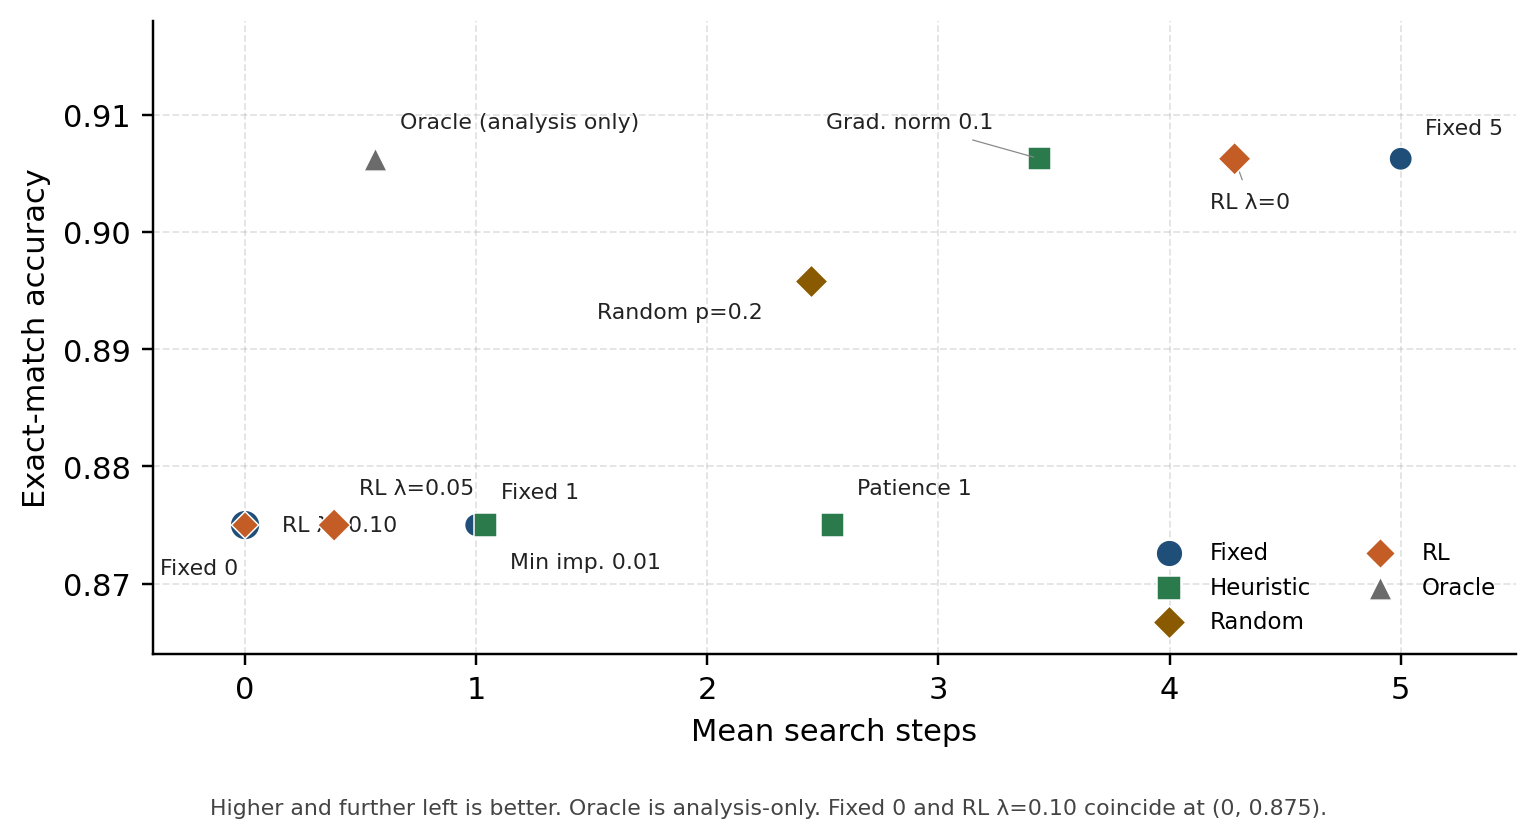
\includegraphics[width=0.84\textwidth]{figures/controller_tradeoff.png}
\caption{Accuracy--compute tradeoff ($M{=}96$ episodes; $x$: mean search steps;
$y$: exact match; higher/left better). Oracle is analysis-only.
Fixed~0 and RL~$\lambda{=}0.10$ coincide at $(0,0.875)$. Source:
\texttt{report/data/controller\_tradeoff.csv}.}
\label{fig:tradeoff}
\end{figure}

\noindent Figure~\ref{fig:tradeoff}: Fixed~5, gradient-norm~$0.1$, and
RL~$\lambda{=}0$ share exact match $0.90625$; gradient norm is further left
($3.438$ vs.\ $4.281$); RL is $0.719$ steps left of Fixed~5;
$\lambda\in\{0.05,0.10\}$ move left and down to $0.87500$; the oracle is far
left but not deployable. No smooth Pareto claim from these points.

\begin{figure}[H]
\centering
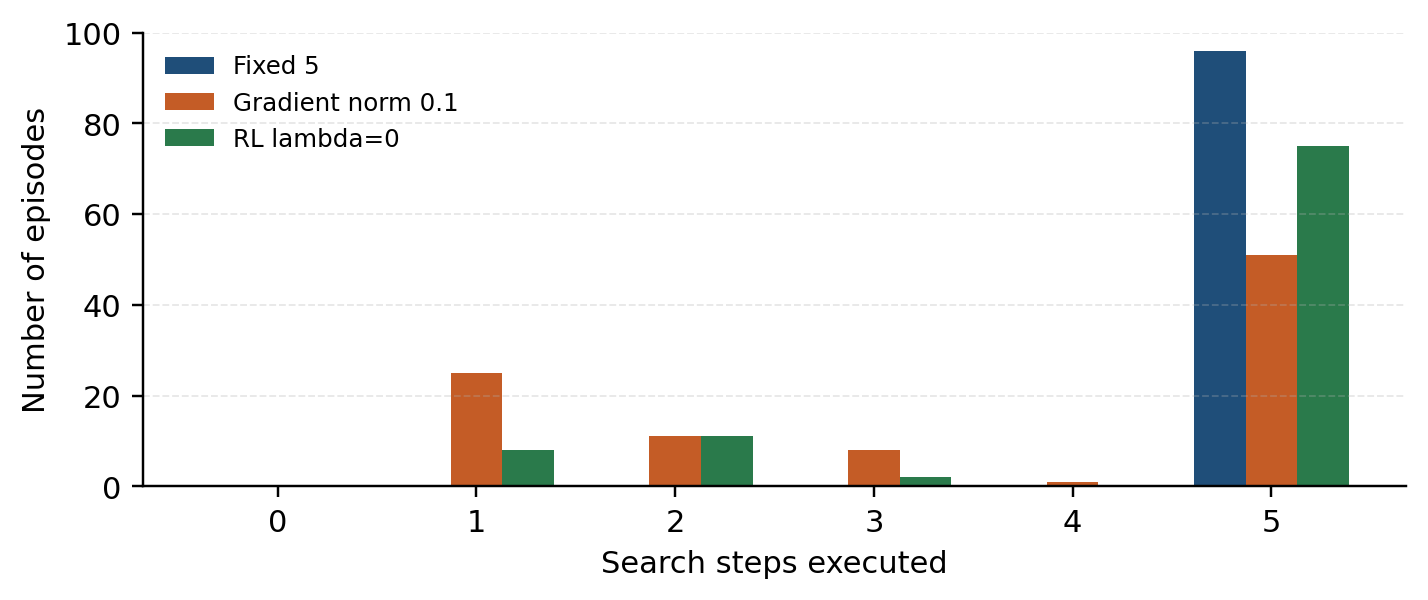
\includegraphics[width=0.78\textwidth]{figures/stopping_distribution.png}
\caption{Stopping-step histogram (episode counts over $M{=}96$; bins $0$--$5$;
deterministic $p(\texttt{stop})\ge0.5$; correlated LOO episodes). Source:
\texttt{report/data/stopping\_distribution.csv}.}
\label{fig:hist}
\end{figure}

Figure~\ref{fig:hist}: the RL reduction is concentrated, not broad
($75/96$ episodes still use five steps, vs.\ $51/96$ for gradient norm and
$96/96$ for Fixed~5).

\paragraph{Main result, in order.}
(1)~RL is operational.
(2)~It transfers from checkpoints~0,~1 to checkpoint~2.
(3)~RL~$\lambda{=}0$ matches Fixed-5 exact match ($0.90625$).
(4)~It uses fewer mean steps than Fixed~5 ($4.281$ vs.\ $5.000$).
(5)~It does not beat gradient-norm stopping ($3.438$ steps at the same exact
match).
(6)~Larger $\lambda$ collapses to premature stopping.
(7)~Limited \texttt{pattern\_2d} proof of concept.

\paragraph{Oracle analysis.}
$T^\star=\min\{t\in\{0,\ldots,H\}:\widehat{y}_t=y_{\mathrm{query}}\}$ on
success; else stop at $H$ ($9=96\times(1-0.90625)$ failures at step~$5$).
Mean steps $0.562$ is analysis-only at matched exact match; the gap to $4.281$
shows poor earliest-correct identification. Not deployable.

\FloatBarrier
% =====================================================================
\section{Discussion}
% =====================================================================

Fixed-5 works because deterministic search often repairs imperfect encoder
initialization (exact match $0.87500\to0.90625$).
Simple rules fail because support score and gradient norm are imperfect proxies
for query exact match.
RL improves only modestly, plausibly from linear capacity, weak observations,
sparse reward, REINFORCE variance, a small length-8 training split, checkpoint
shift, and a coarse $\lambda$ grid.
Gradient norm may align better with this checkpoint and task subset; we do not
claim that ranking will generalize.
Validation selected $\lambda{=}0$; larger penalties preferred cheap incorrect
termination.
The result remains useful as a complete software and evaluation path for richer
controllers.

Next, ranked:
(a)~fine $\lambda$ grid $0.001$--$0.02$;
(b)~multiple policy seeds;
(c)~length-96 held-out evaluation;
(d)~task-level bootstrap;
(e)~supervised earliest-correct diagnostic;
(f)~small MLP policy;
(g)~richer label-free observations;
(h)~ARC only with a provenance-clear checkpoint.
Not immediate: PPO.

\paragraph{Limitations.}
\texttt{pattern\_2d} only; in-family; 24 tasks / 96 correlated LOO episodes;
one held-out checkpoint; weak policy-seed analysis; coarse $\lambda$ sweep;
selected $\lambda{=}0$; no uncertainty; RL dominated by gradient norm;
offline trajectories; no ARC; no OOD claim.

\FloatBarrier
\Needspace{14\baselineskip}
% =====================================================================
\section{AI Assistance and Process}
% =====================================================================

AI assistance was used during implementation, debugging, documentation, and
diagnostic review.
I directed the research question, experimental design, interpretation, and
final scientific decisions, and verified every reported claim against persisted
code and artifacts.
The repository postmortem records the main experimental decisions, failures,
and corrections in chronological order.

% =====================================================================
\section{Conclusion}
% =====================================================================

A minimal RL stop-or-continue controller was successfully integrated into LPN
latent search.
On the held-out checkpoint experiment, it matched Fixed-5 exact match with a
modest reduction in average search steps.
It did not outperform the strongest tested heuristic.
The result provides a rigorous prototype and motivates better observations,
training objectives, and larger evaluation protocols.

\clearpage
\bibliographystyle{plain}
\bibliography{references}

\end{document}
